\chapter{Evaluation}\label{chap:evaluation}
Through the use of the framework described in the previous chapter, we evaluate four different algorithms for next-activity prediction side-by-side: Two implementations that mimic the networks by Evermann et al. and Schönig et al, and the PFS and SP2 approaches presented in \autoref{chap:taking-inspiration}. The reimplementation of Evermann's and Schönig's approaches will be referred to as EVM and SCH respectively. For each model, we will analyze the four different approaches for structuring the training data for performance differences from \autoref{chap:training-framework}.

First we justify our choice of datasets in \autoref{sec:eval:dataset-choice}. As we follow the KDD process, we then lead through the data pre-processing and transformation phases in \autoref{sec:eval:data-preprocessing} and \autoref{sec:eval:data-transformation}. The latter section also covers the strategy used to engineer the features for the SP-2 and PFS models.
Then, the test setup and the used training strategy is presented in \autoref{sec:eval:test-setup}, followed by the set of criteria by which we judge the results in \autoref{sec:eval:criteria}. Finally, the chapter ends with the presentation in \autoref{sec:eval:results} and discussion of the results in \autoref{sec:eval:discussion}. Used and relevant technologies are highlighted in each sections.

\section{Choice of datasets}
\label{sec:eval:dataset-choice}
In \autoref{sec:intro:contribution}, we criticized the great variety of datasets used to evaluate approaches in Predictive Process Monitoring. While we can not establish a standard, we ensure comparability of our results to a variety of works by evaluating the four models on seven datasets in total, coming from the following sources:

\begin{itemize}
    \item BPIC11, an event log from cases in a Gynaecology department of a Dutch Academic Hospital~\cite{BPIC2011}
    \item BPIC12, an event log for loan and overdraft applications from a Dutch Financial Institute~\cite{BPIC2012}
    \item BPIC15 is divided into five logs. Each contains all building permit applications over a period of approximately four years from a Dutch municipality. They are referred to as BPIC15-1 to BPIC15-5 in the following~\cite{BPIC2015}
\end{itemize}

We picked the three BPIC datasets as we believe that they cover a spectrum of process complexity. The least complex end of it is marked by BPIC12, which covers a loan application process from a financial institution with a small variance in trace length and a very small number of different activities. The complex end is marked by BPIC11, which covers patient treatments in a hospital. This results in logs of longer traces and an especially high number of distinct activities. BPIC15 resides relatively in the middle of the two, as \autoref{tab:dataset-characteristics} indicates.

While process models were easily mined for BPIC12~\cite{adriansyah2012mining}, they were more complex for BPIC15~\cite{van2015benchmarking}, and barely obtained for BPIC11. Furthermore we take the increasing number of distinct activities and variance in trace length to be measures of complexity.

Furthermore, these datasets allow us to compare our findings to the following works, which also worked on next-element predictions. When comparing, it is important to differentiate between the works that focused on case-specific predictions like us and those that focused on whole event streams:

\begin{itemize}
    \item Predicting the next element in a stream, not specific to a case
    \begin{itemize}
        \item BPI12: Tax et al.~\cite{tax2017}
        \item BPI12: Evermann et al.~\cite{evermann2016}
    \end{itemize}
    \item Predicting the next element for a specific case
    \begin{itemize}
        \item BPI12: Böhmer et al.~\cite{boehmer2018probability}
    \end{itemize}
\end{itemize}

\begin{table}[]
\centering
\begin{tabular}{lrrrrrrr}
\textbf{Dataset} & \textbf{min TL} & \textbf{max TL} &  \textbf{mean TL} & \textbf{Traces} & \textbf{Events} & \textbf{Activities} \\
\hline
\textbf{BPIC12} & 3 & 96 & 12.56 & 13 087 & 164 506 & 23\\
\textbf{BPIC15-1} & 2 & 101 & 43.55 & 1199 & 52 217 & 398\\
\textbf{BPIC15-2} & 1 & 132 & 53.31 & 832 & 44 354 & 410\\
\textbf{BPIC15-3} & 3 & 124 & 42.35 & 1409 & 59 681 & 383\\
\textbf{BPIC15-4} & 1 & 116 & 44.91 & 1053 & 47 293 & 356\\
\textbf{BPIC15-5} & 6 & 154 & 51.10 & 1156 & 59 083 & 389\\
\textbf{BPIC11} & 1 & 1 814 & 131.49 & 1 143 & 150 291 & 524\\
\end{tabular}
\caption[Trace properties in each dataset]{Properties of the traces contained in the used datasets. TL abbreviates trace length.}
\label{tab:dataset-characteristics}
\end{table}

\section{Data pre-processing}
\label{sec:eval:data-preprocessing}
In the first step of the KDD process~\cite{fayyad1996data}, the data is pre-processed to prepare the data for our prediction use case and eliminate generally known properties that hinder machine learning model performance. In our case, this encompassed two steps for all datasets:

\begin{enumerate}
    \item Filter for completed events
    \item Drop all columns which exhibit zero entropy, i.e. which contain only a single value
    \item Eliminate features which correlate strongly. To account for categorical correlation, the bias-corrected version of Cramér's~V~\cite{bergsma2013bias} is used.
\end{enumerate}

\autoref{tab:dataset-preprocessing} illustrates which features were removed and which ones were kept after the three steps.

In step 1, the lifecycle:transition feature was filtered so that only completed events were left. This was done to reduce dimensionality and improve comparability, since BPIC11 only contains completed events.

In step 2, the transition feature was removed in every dataset, since it had been filtered before. No other features exhibited zero entropy.

In step 3, the results from the pairwise application of Cramér's~V~\cite{bergsma2013bias} on the features in a dataset reveal that some features correlate strongly with several others in the BPIC11 and BPIC15 datasets. The respective heatmaps can be found in \autoref{appendix:correlation-heatmaps}. Thus, these were dropped. As evidenced in the respective heatmap, the BPIC12 dataset with its small number of features did not require any removals.

\begin{table}
\centering
\begin{tabular}{lp{6cm}p{6cm}}
\textbf{Dataset} & \textbf{Omitted features} & \textbf{Remaining features}\\
\hline
\textbf{BPIC11} & lifecycle:transition, Producer code, Activity code, Specialism code & time:timestamp, concept:name, org:group, Number of executions, Activity code, Producer code, Specialism code, Section\\
\textbf{BPIC12} & lifecycle:transition & org:resource, concept:name, time:timestamp\\
\textbf{BPIC15} & lifecycle:transition, activityNameNL, activityNameEN, action\_code, dueDate & time:timestamp 	dateFinished 	planned 	concept:name 	monitoringResource 	org:resource 	question
\end{tabular}
\caption{Omitted features during pre-processing}
\label{tab:dataset-preprocessing}
\end{table}

The activities described above were conducted in JupyterLab notebooks~\cite{web:jupyter}, where Anaconda~\cite{web:anaconda} was used to create a stable development environment. The OpyenXes~\cite{web:opyenxes} library proved to be especially useful for transferring raw XES logs into workable Pandas dataframes.

\section{Data transformation}
\label{sec:eval:data-transformation}
Having removed unneeded features, the remaining ones were encoded following common procedures. Timestamps were converted to numerical features for each trace, i.e. each timestamp $t_i$ was made relative to the beginning of a trace by calculating $t_i - t_0$. Each numerical feature $x$ was normalized with values specific to each trace using the min-max method:

$$normalize(x) =
\begin{cases}
\frac{x-min(x)}{max(x)-min(x)} & \text{if } min(x) \neq max(x)\\
1 & \text{otherwise}
\end{cases}
$$

Categorical features without ordinal properties, i.e. all of the remaining features, were encoded using one-hot encoding if possible. In the case of the input for the EVM model, the concatenation of activity name and resource ID was encoded with dictionary encoding, as demonstrated in his paper~\cite{evermann2016}. Furthermore, the additional SP-2 and sub-sequence features needed to be engineered, which the following subsection show.

\subsection*{SP-2 feature engineering}
For every trace, SP-2 features mark whether an activity has occured yet. Thus, these features are engineered in an iterative fashion, as \autoref{lst:sp2-generation} outlines. For every trace, a new feature vector \texttt{sp2\_df} is created and the occurence of the first activity is marked inside it. Now, a loop begins over the remaining steps, where each previous row inside \texttt{sp2\_df} is copied into the currently indexed row and the presence of the current activity is marked. This repeats itself until the trace has been processed completely.

\begin{listing}[ht]
\begin{minted}{python}
# Dataframe initialization with zeroes
sp2_df = pd.DataFrame(columns=activity_labels,
                      index=range(0,len(t)),
                      dtype=np.bool)
for col in sp2_df.columns: sp2_df[col].values[:] = 0

# mark first occuring SP-2
cname = "{0}{1}".format(sp2_prefix, t[target_col][0])
sp2_df[cname].values[0]  = 1

# copy over values from last row and
# set activity labels accordingly
for i in range(1,len(t)):
    first_activity_name = t["concept:name"].iloc[i]
    col = "{0}{1}".format(sp2_prefix,first_activity_name)

    sp2_df.values[i] = sp2_df.values[i-1]
    sp2_df[col].values[i] = 1
\end{minted}
\caption{Generating SP-2 features for a single trace \texttt{t} and a specific target column \texttt{target\_col}.}
\label{lst:sp2-generation}
\end{listing}

\subsection*{Sub-sequence feature engineering}
The sub-sequence features for the PFS model were created with the help of the PrefixSpan algorithm implementation from the \textit{prefixspan-py} library~\cite{web:prefixspan-py}. As \autoref{lst:pfs-mining} shows, the library greatly facilitates obtaining closed sub-sequences ranked by support, returning a two-dimensional array of sub-sequences, with one array per sub-sequence. The sequences are mined from the entirety of traces, and we pick the top 25 sequences as features to be encoded.

\begin{listing}[ht]
\begin{minted}{python}
prefixspan_traces = PrefixSpan(encoded_traces)
closed_sequences = prefixspan_traces.topk(25, closed=True)
\end{minted}
\caption{Obtaining closed sequences using the \textit{prefixspan-py} library.}
\label{lst:pfs-mining}
\end{listing}

After mining the sequences, a loop is executed for every trace, shown in \autoref{lst:subsequence-feature-creation}. For each index \verb=i= it is checked whether any of the mined sub-sequences starts at that position. This is checked by peeking ahead of \verb=i= for the length of the sub-sequence. As in the case of the SP-2 features, the occurence of a sub-sequence is marked with a boolean flag in the feature vector \verb=subseq\_df= from the row that it occured in onwards.

\begin{listing}[ht]
\begin{minted}{python}
subseq_df = pd.DataFrame(columns=subseq_labels,
                         index=range(0,len(t)),
                         dtype=np.bool)
subseq_df[:].values[:] = False
activity_codes = t[target_col].map(event_to_int)
tlen = len(t)

for i in range(0, tlen):
  # loop through all sub-sequences
  for subseq_idx, subseq in enumerate(ps):
    if tlen <= i+len(subseq): continue

    # check if subseq takes place in the following steps
    subsequence_found = True
    j = 0

    while subsequence_found and j < len(subseq):
      if subseq[j] != activity_codes[j+i]:
        subsequence_found = False
        j += 1

    # if subseq took place, subsequence_found is still true
    if subsequence_found:
      subseq_df.values[j+i:,subseq_idx] = True
\end{minted}
\caption{Enriching a trace \texttt{t} with sub-sequence features by detecting those that are contained inside it.}
\label{lst:subsequence-feature-creation}
\end{listing}

\subsection*{Target construction}
For each itemset $i_t$ at a given timestep $t$, the prediction target $a_{t+1}$ was constructed. While the itemset could also contain data attributes, the prediction target solely consisted of the activity name. For the target of the last $t$ of a trace, a marker for denoting the end of the sequence, \verb=EOS=, was introduced.
As the goal is to predict the next activity, the column containing this information needed to be identified in the data. For all datasets, this turned out to be \verb=concept:name=.

\section{Test setup}
\label{sec:eval:test-setup}
To conduct the experiments, Docker containers were built with the development Anaconda environment inside them~\cite{web:docker}. Using a version of Docker for GPU applications running on NVIDIA hardware~\cite{web:nvidia-docker}, each network-batch-formatting combination was trained and evaluated on a single NVIDIA K80 GPU of the HPI FutureSOC Lab~\cite{web:fsoc} so that multiple models could be trained and evaluated simultaneously. The complete source code used for evaluation is publicly available on GitHub at \href{https://github.com/flxw/master-thesis-code}{flxw/master-thesis-code}.\\

All datasets were split into training and test sets of complete traces. While $25\%$ of the traces were used for validation and testing, the remaining $75\%$ were used for training purposes. The sets were shuffled and stratified to contain an approximately similar distribution of trace lengths.

A model was saved when its validation loss, calculated on the test set, hit a new record low. If the validation loss did not improve for 10 epochs, the training was stopped. This technique is commonly referred to as early stopping and helps avoid overfitting. \autoref{tab:training-setup} shows information about the training setup of the networks side-by-side. Additionally, the number of samples per batch is shown in \autoref{tab:batch-sizes}.

\begin{table}[ht!]
    \centering
    \begin{tabular}{lcccc}
        \textbf{Network}   & \textbf{EVM} & \textbf{SCH} & \textbf{SP2} & \textbf{PFS}\\
        \hline
        \textbf{Optimizer} & SGD & \multicolumn{3}{c}{RMSprop} \\
        \textbf{Loss}      &\multicolumn{4}{c}{Categorical crossentropy}\\
        \textbf{Weight initializer} & Zeros & None & \multicolumn{2}{c}{Glorot normal}\\
        \textbf{Epochs}    & 50 & 100 & 150 & 150\\
        \textbf{Features}  & \makecell{Activity +\\Resource} & \multicolumn{3}{c}{All usable data attributes}\\
    \end{tabular}
    \caption[Used hyper-parameters for each model]{Used hyper-parameters for each model, with the number of epochs to be understood as the maximum number of epochs, as training may stop early}
    \label{tab:training-setup}
\end{table}

\marginpar{SGD abbreviates Stochastic Gradient Descent. Additionally, during EVM model training, the learning rate decay is set to $0.75$ at the $25^{th}$ epoch.}

\begin{table}
\centering
\begin{tabular}{c|rrrr}
Dataset & Individual & Grouped & Padded & Windowed \\
\hline
BPIC11    & 1 & & 7 & 1054\\
BPIC 12   & 1 & & 89 & 939\\
BPIC 15-1 & 1 & & 9 & 365\\
BPIC 15-2 & 1 & & 5 & 316\\
BPIC 15-3 & 1 & & 10 & 414\\
BPIC 15-4 & 1 & & 8 & 334\\
BPIC 15-5 & 1 & & 7 & 420\\
\end{tabular}
\caption[Batch sizes for each dataset and strategy]{Number of traces per batch for the different datasets and batching strategies}
\label{tab:batch-sizes}
\end{table}

\section{Evaluation criteria}
\label{sec:eval:criteria}
The following three metrics are the focus in the evaluation of the sixteen model-formatting combinations:

\begin{enumerate}
    \item\textbf{Accuracy} - The share of correct next-activity predictions.
    \item\textbf{Resource consumption} - The amount of time and memory required during training.
    \item\textbf{Stability} - Whether the prediction accuracy changes as the trace progresses.
\end{enumerate}

While the first two criteria target the general usability of each model, the last one permits making a judgment about the stability of the predictions. It is inspired by the works of Francescomarino et al.~\cite{francescomarino2015} and Klinkmüller et al.~\cite{klinkmuller2018reliablemonitoring}. This allows better insights into how prediction accuracy develops over time, and facilitates building trust in the model, as indicated in the introduction of the thesis.

\section{Results}\label{sec:eval:results}
The three aforementioned criteria were applied to each model-batching combination on each dataset, and the results are presented in this section. By evaluation criterion, we go through the measurements. Some of the corresponding figures can be found in \autoref{appendix:evaluation-measurements}, due to space reasons.

\subsection*{Accuracy}
The overall accuracy is a good indicator of the prediction performance of any prediction model. In this section we will go over the model performances per batching strategy and explain the results. In \autoref{fig:max-accuracies-bpic2011} to \autoref{fig:max-accuracies-bpic2015-5}, the model performances per dataset are presented, grouped by batching strategy. The plots make apparent that only three models perform well consistently and that all react very differently to each batching strategy.

Looking at the performance of the EVM model across all datasets, it is evident that it is consistently outperformed. Its performance on the BPIC12 datasets represents an exception. We trace this lack of performance back to the application of an Embedding layer, which we suspect to require more data than included in most datasets to improve its internal data representation. The performance jump on the BPIC12 dataset corresponds nicely to the small number of activities and large number of traces in \autoref{tab:dataset-characteristics}, which helps the Embedding learn better.

Unsurprisingly, the individual batching strategy often results in slightly worse accuracies than the grouped batching strategy, with the exception of the BPIC12 dataset. We trace this back to the frequent adjustment of weights that might lead the loss optimization into local minima. In the trace length distributions in \autoref{appendix:trace-length-distributions}, the explanation for the high accuracy on BPIC12 with the individual batching strategy can be found. As this dataset has the highest number of traces and a relatively even distribution of lengths, the batches become too large, leading to lost optimization opportunities. With this knowledge, the strategy should be enhanced to split batches if they exceed a certain size threshold.

The padded strategy leads to consistently good results throughout the datasets and only loses accuracy on the BPIC11 datasets where the training set had to be shrunk because traces exceeded the length threshold.

While the batching strategies that provide the whole history to the model consistently see the SCH, SP2 and PFS models on par with at most $0.1$ difference, the windowed batching strategy leads to very different results depending on the dataset and the model. With the window size of three suggested by Schönig et al., the model does not have many timesteps to learn from in any given sample. However, this loss of information does not impact the SP2 model. We assume that its SP-2 features encode the history that is cut away and thus help it come close to the general maximum accuracy of the dataset with the exception of BPIC11.

\begin{figure}
    \centering
    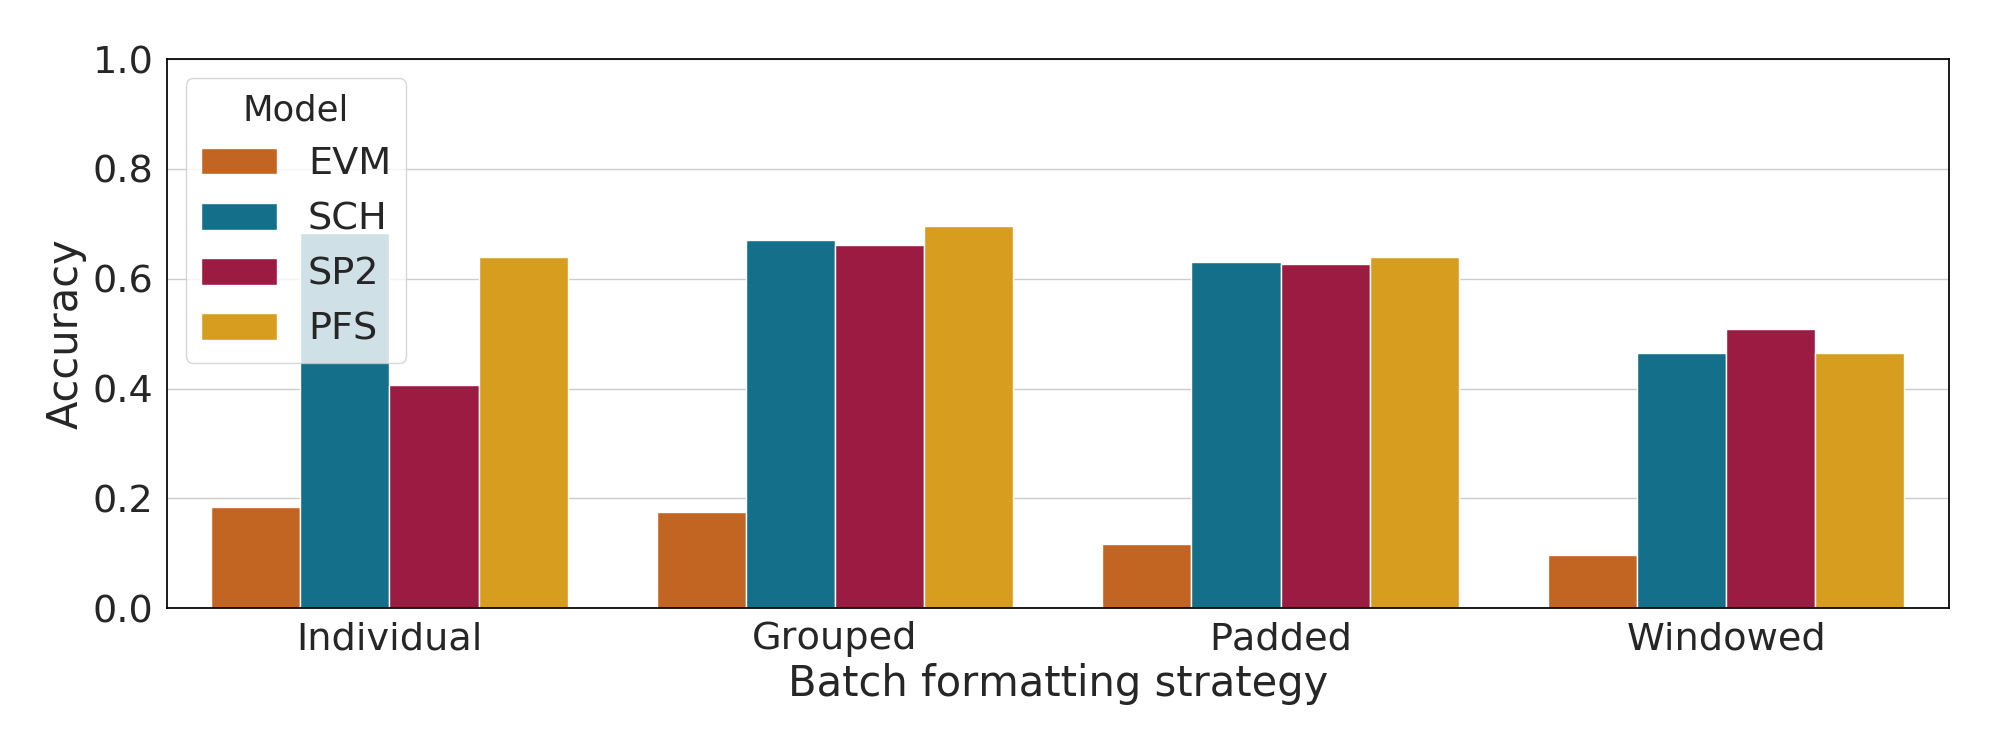
\includegraphics[width=\textwidth]{gfx/bpic2011/accuracies.png}
    \caption{Best accuracies on the validation set of BPIC11}
    \label{fig:max-accuracies-bpic2011}
\end{figure}
\begin{figure}
    \centering
    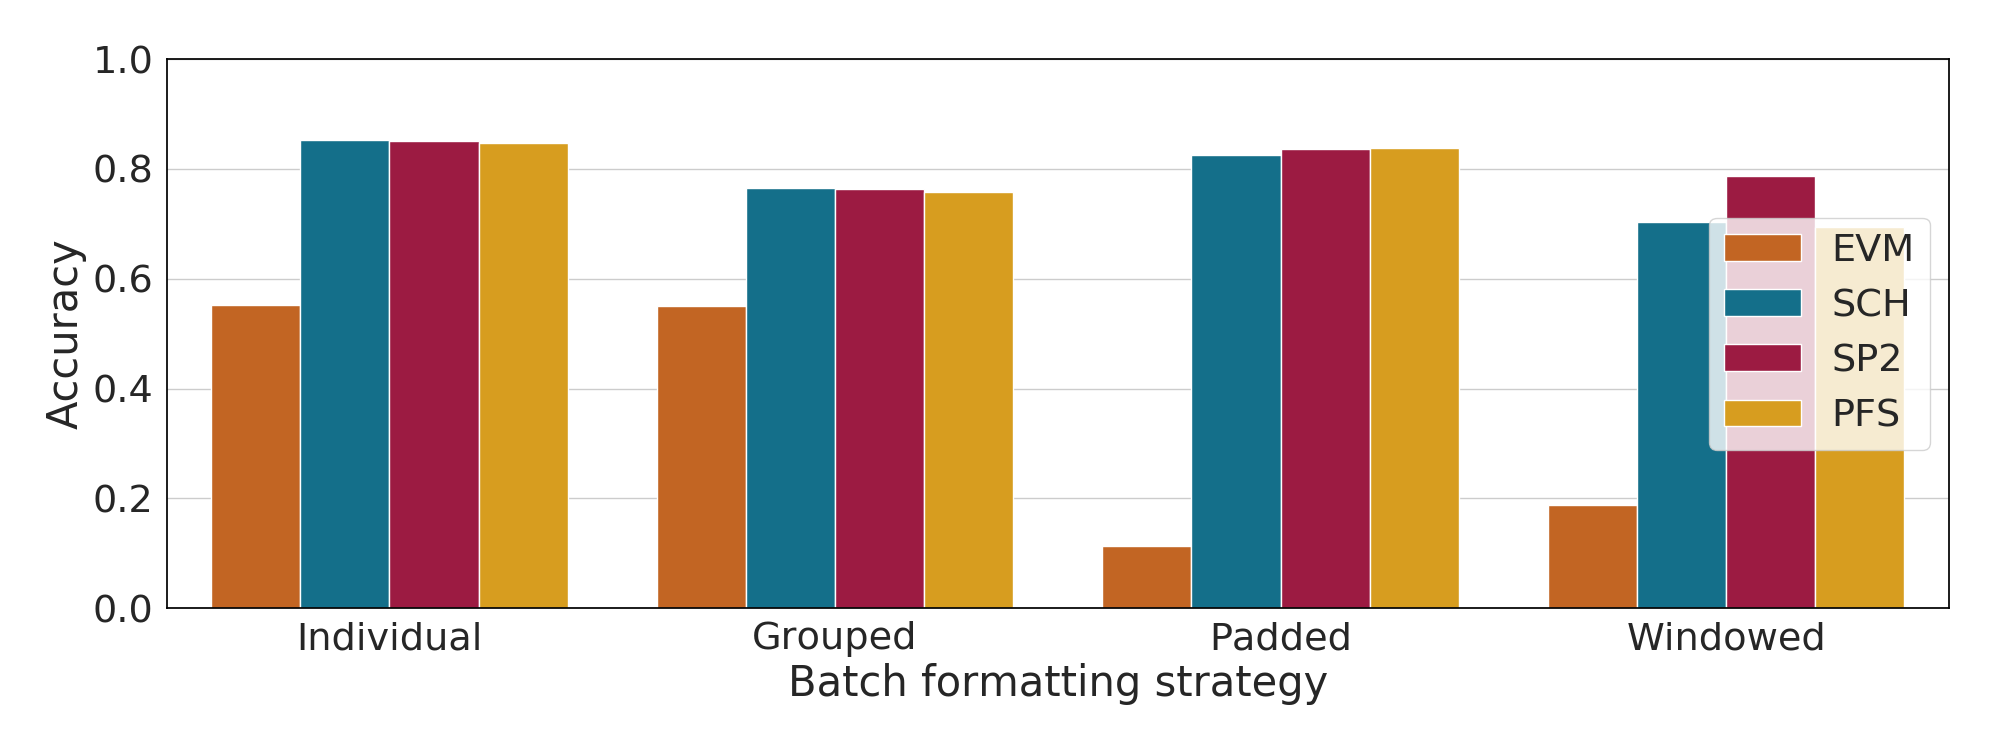
\includegraphics[width=\textwidth]{gfx/bpic2012/accuracies.png}
    \caption{Best accuracies on the validation set of BPIC12}
    \label{fig:max-accuracies-bpic2012}
\end{figure}
\begin{figure}
    \centering
    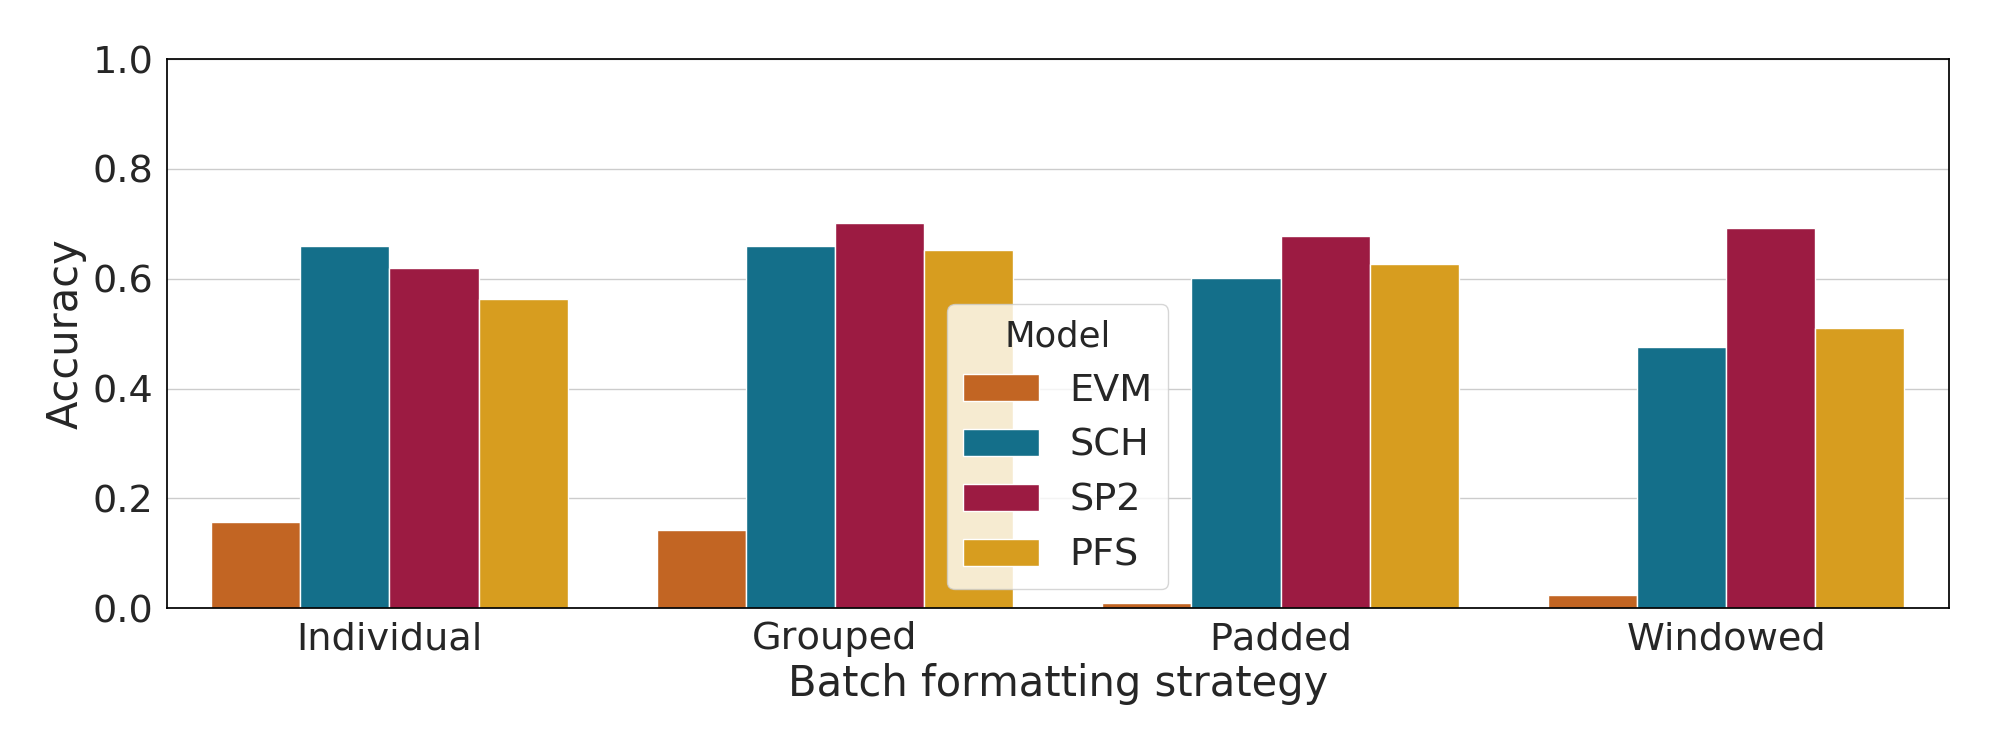
\includegraphics[width=\textwidth]{gfx/bpic2015_1/accuracies.png}
    \caption{Best accuracies on the validation set of BPIC15-1}
    \label{fig:max-accuracies-bpic2015-1}
\end{figure}
\begin{figure}
    \centering
    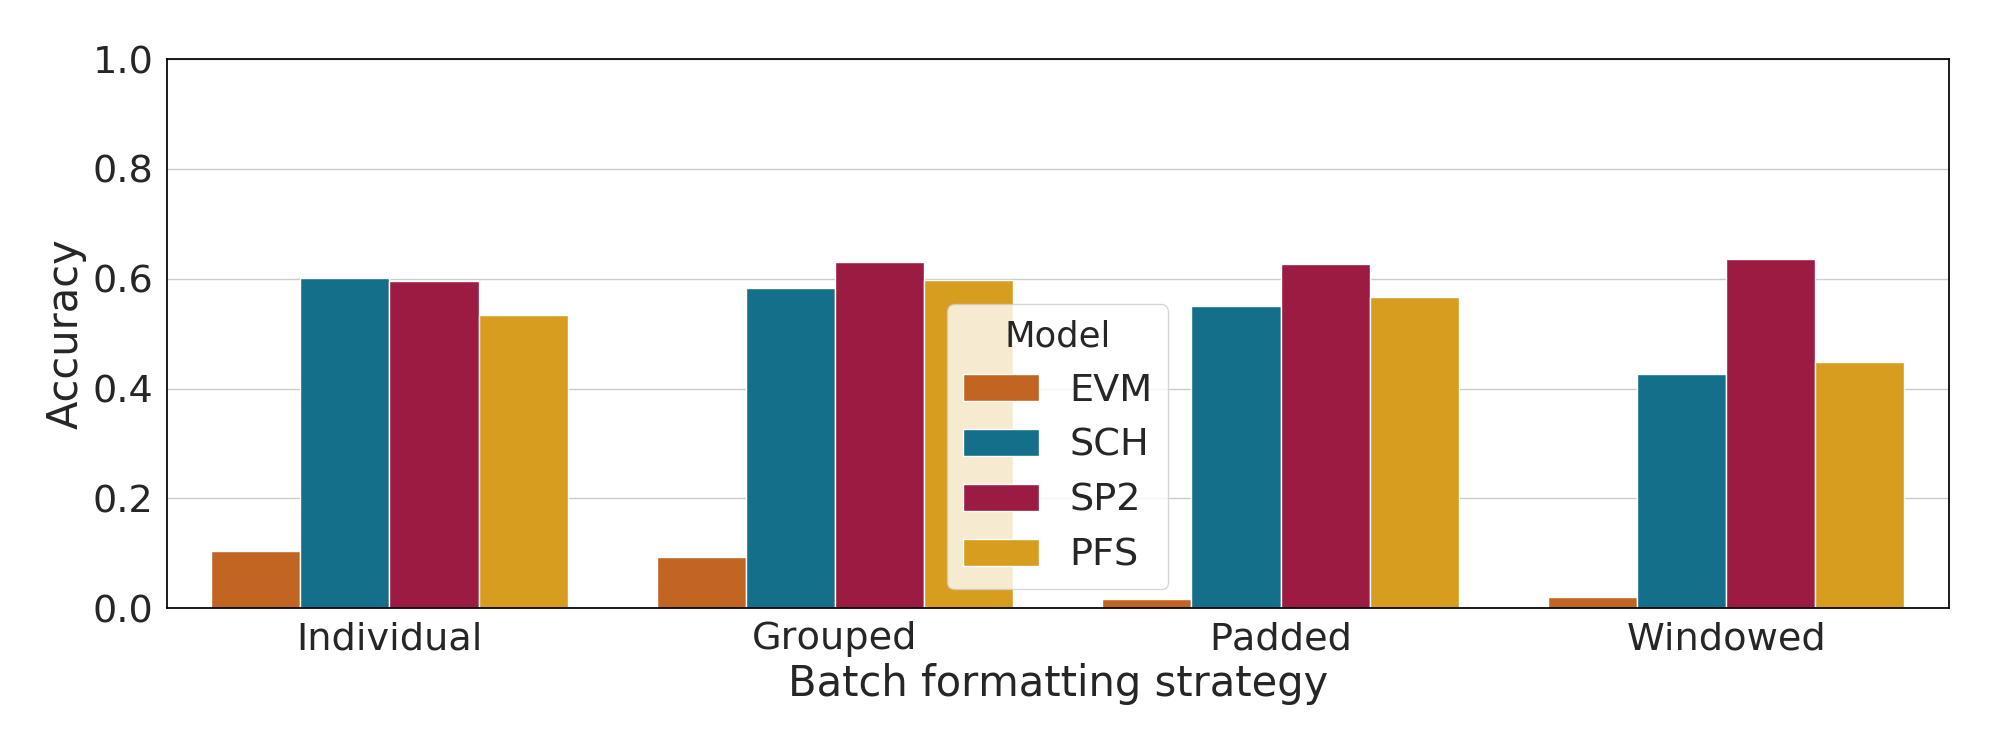
\includegraphics[width=\textwidth]{gfx/bpic2015_2/accuracies.png}
    \caption{Best accuracies on the validation set of BPIC15-2}
    \label{fig:max-accuracies-bpic2015-2}
\end{figure}
\begin{figure}
    \centering
    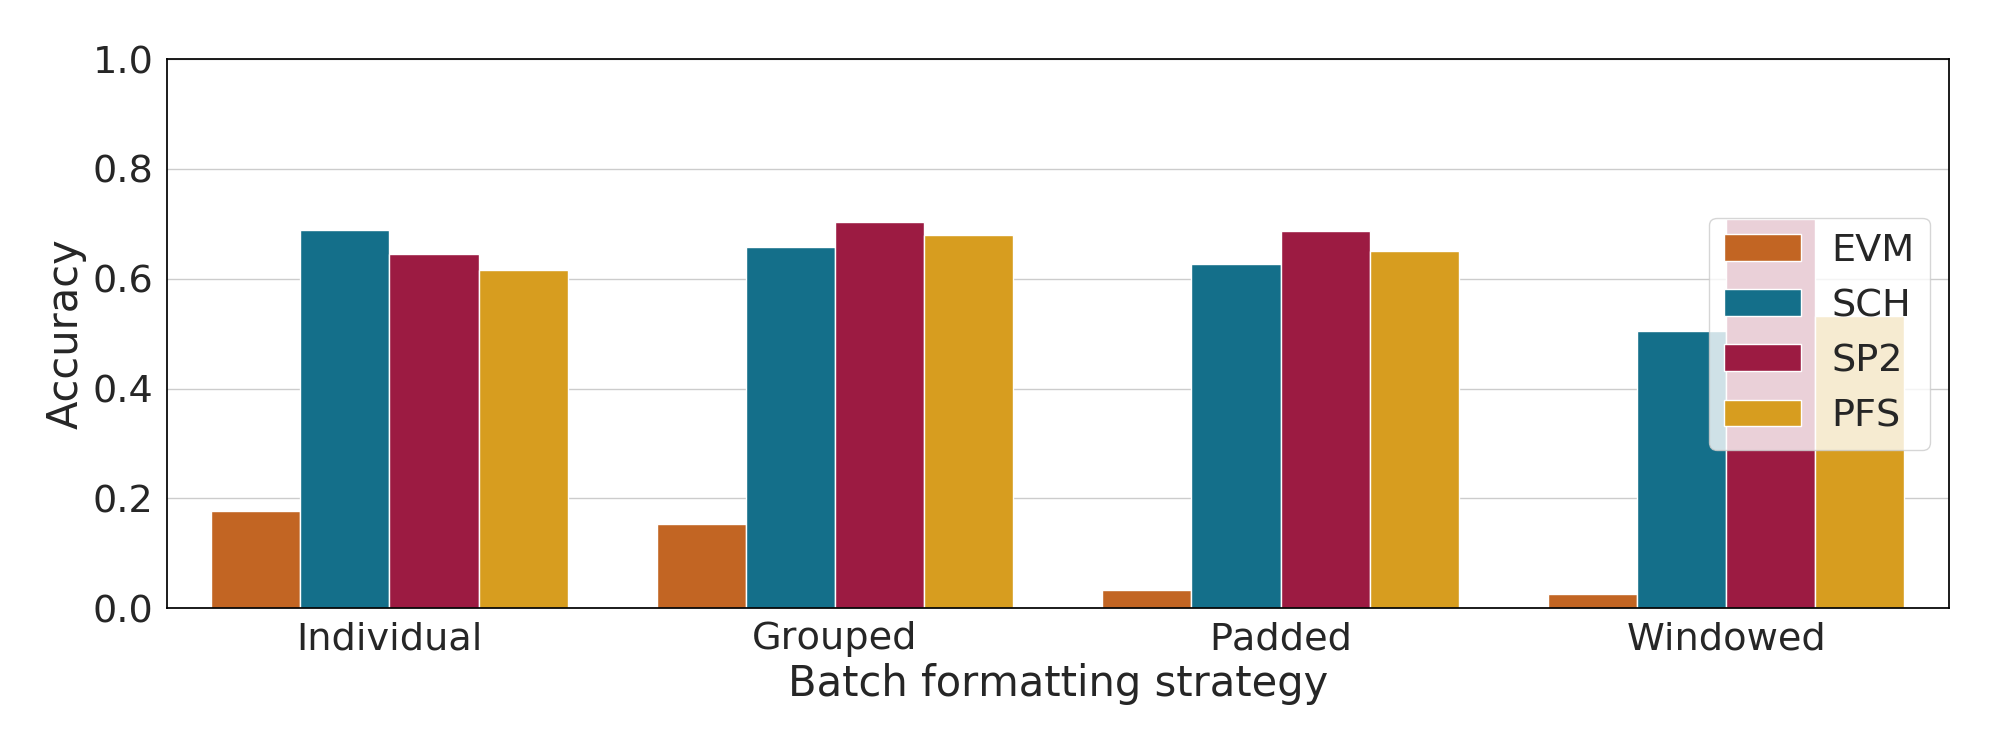
\includegraphics[width=\textwidth]{gfx/bpic2015_3/accuracies.png}
    \caption{Best accuracies on the validation set of BPI15-3}
    \label{fig:max-accuracies-bpic2015-3}
\end{figure}
\begin{figure}
    \centering
    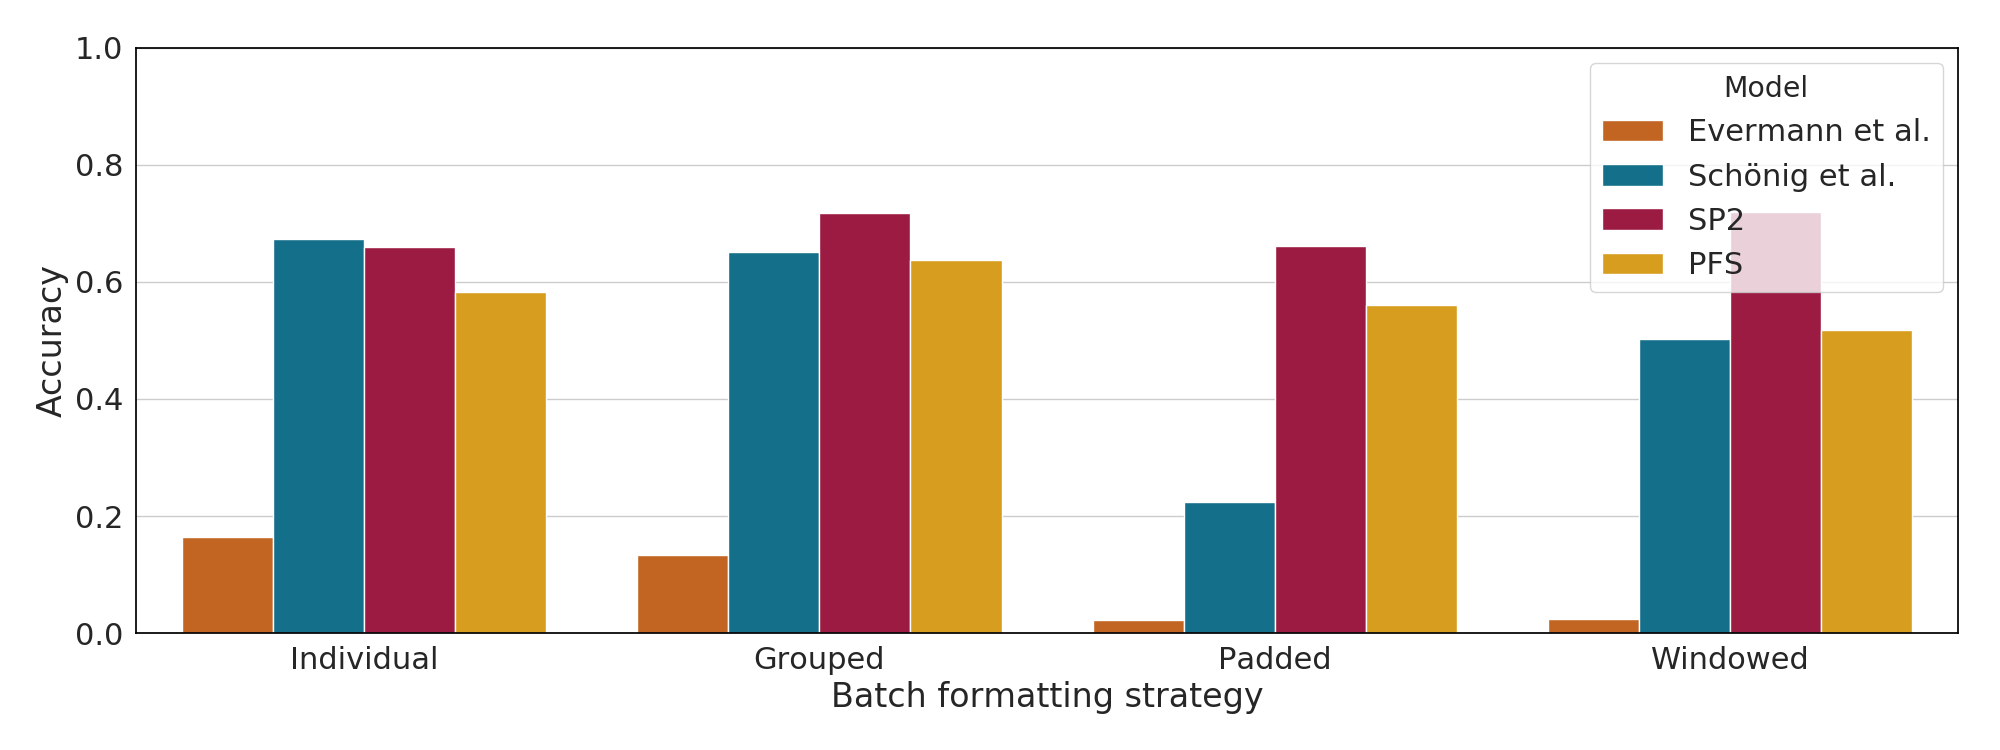
\includegraphics[width=\textwidth]{gfx/bpic2015_4/accuracies.png}
    \caption{Best accuracies on the validation set of BPI15-4}
    \label{fig:max-accuracies-bpic2015-4}
\end{figure}
\begin{figure}
    \centering
    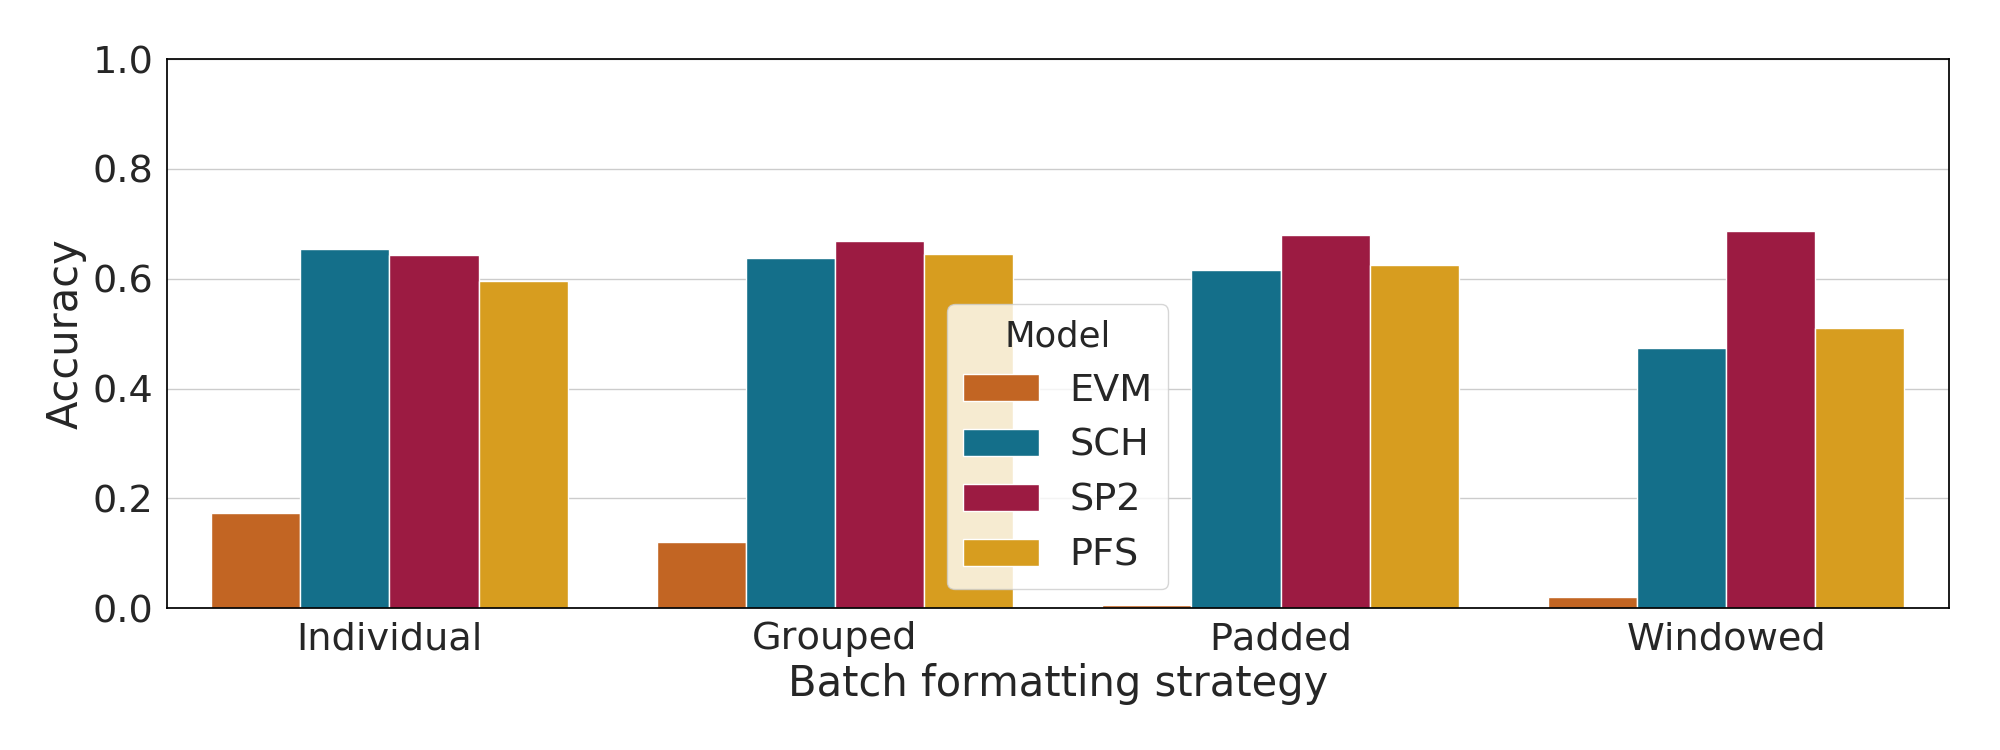
\includegraphics[width=\textwidth]{gfx/bpic2015_5/accuracies.png}
    \caption{Best accuracies on the validation set of BPI15-5}
    \label{fig:max-accuracies-bpic2015-5}
\end{figure}
\FloatBarrier

\subsection*{Training times}
The batch size is an important hyper-parameter, and since it directly corresponds to the number of weight adjustments per epoch, it also impacts the time that the training of an epoch requires. \autoref{fig:BPIC11-training-timings} to \autoref{fig:BPIC15-5-training-timings} illustrate the mean time required for training a model for an epoch, grouped by batching strategy.
In this section we will go over the training times per batching strategy and explain the results.

Unsurprisingly, the individual batching strategy leads to the longest epochs overall. \autoref{tab:dataset-characteristics} reveals that this strategy leads to hundreds of weight adjustments per epoch.

The grouped batching strategy leads to significant reductions in training times, depending on how diverse the trace lengths are. \autoref{tab:dataset-characteristics} explains why the reduction is not as big with BPIC11: It exhibits up to 1814 different lengths, while the other datasets only exhibit $5\%$ to $10\%$ of this number.

With the padded strategy it is possible to overcome the limit imposed by trace lengths and construct batches out of any number of traces. This makes it easier to optimize the batch size, and can thus lead to faster training times. That this does not always lead to better accuracies was shown in the previous section, as e.g. this strategy leads to lost samples on BPIC11.

Finally, the windowing strategy is the fastest by far. It produces a constant number of timesteps and allows for arbitrary batch sizes.

\begin{figure}
    \centering
    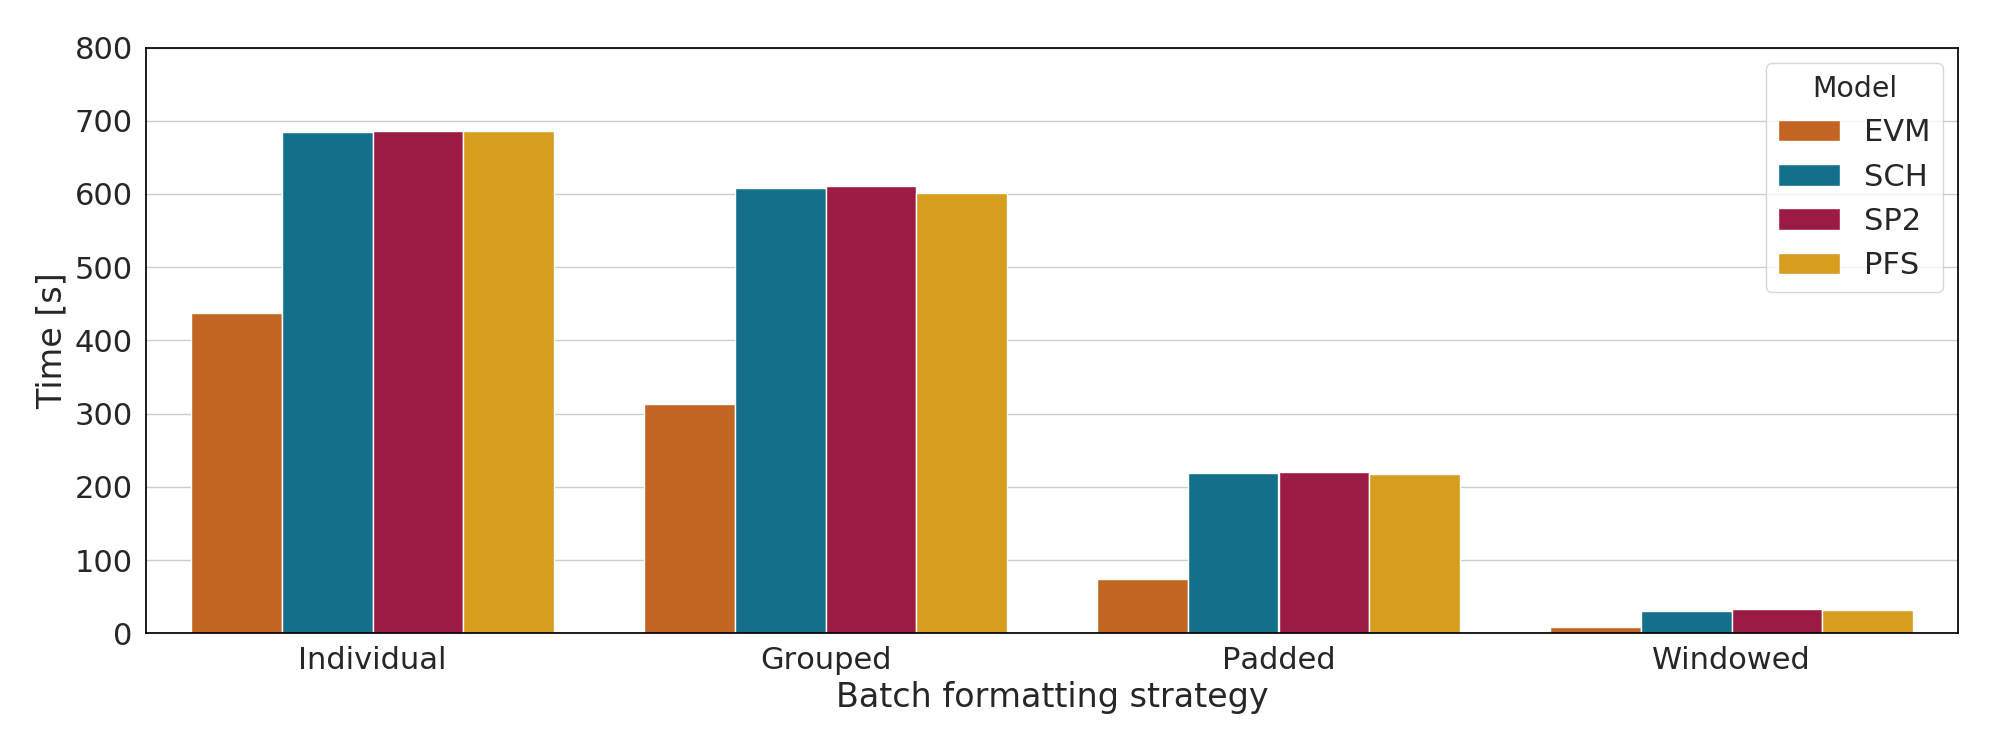
\includegraphics[width=\textwidth]{gfx/bpic2011/train_timings.png}
    \caption{Training times measured on BPIC11}
    \label{fig:BPIC11-training-timings}
\end{figure}
\begin{figure}
    \centering
    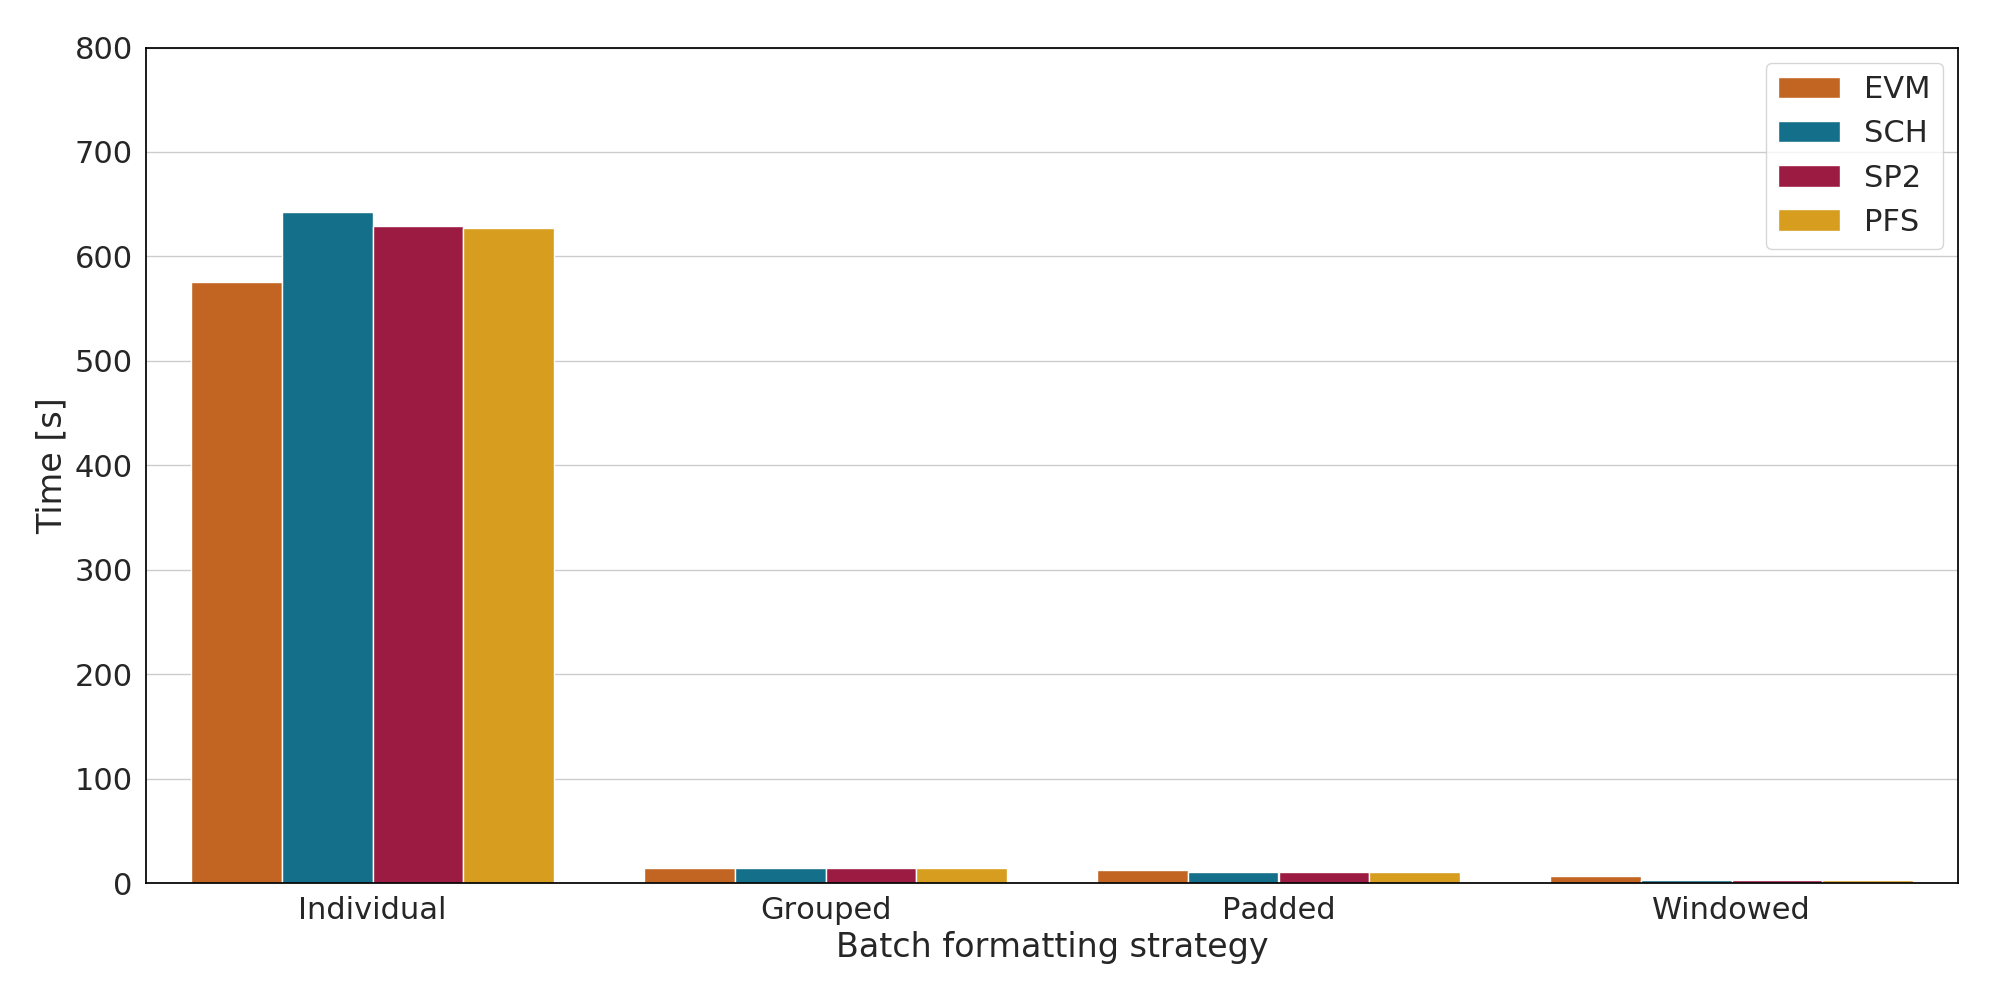
\includegraphics[width=\textwidth]{gfx/bpic2012/train_timings.png}
    \caption{Training times measured on BPIC12}
    \label{fig:BPIC12-training-timings}
\end{figure}
\begin{figure}
    \centering
    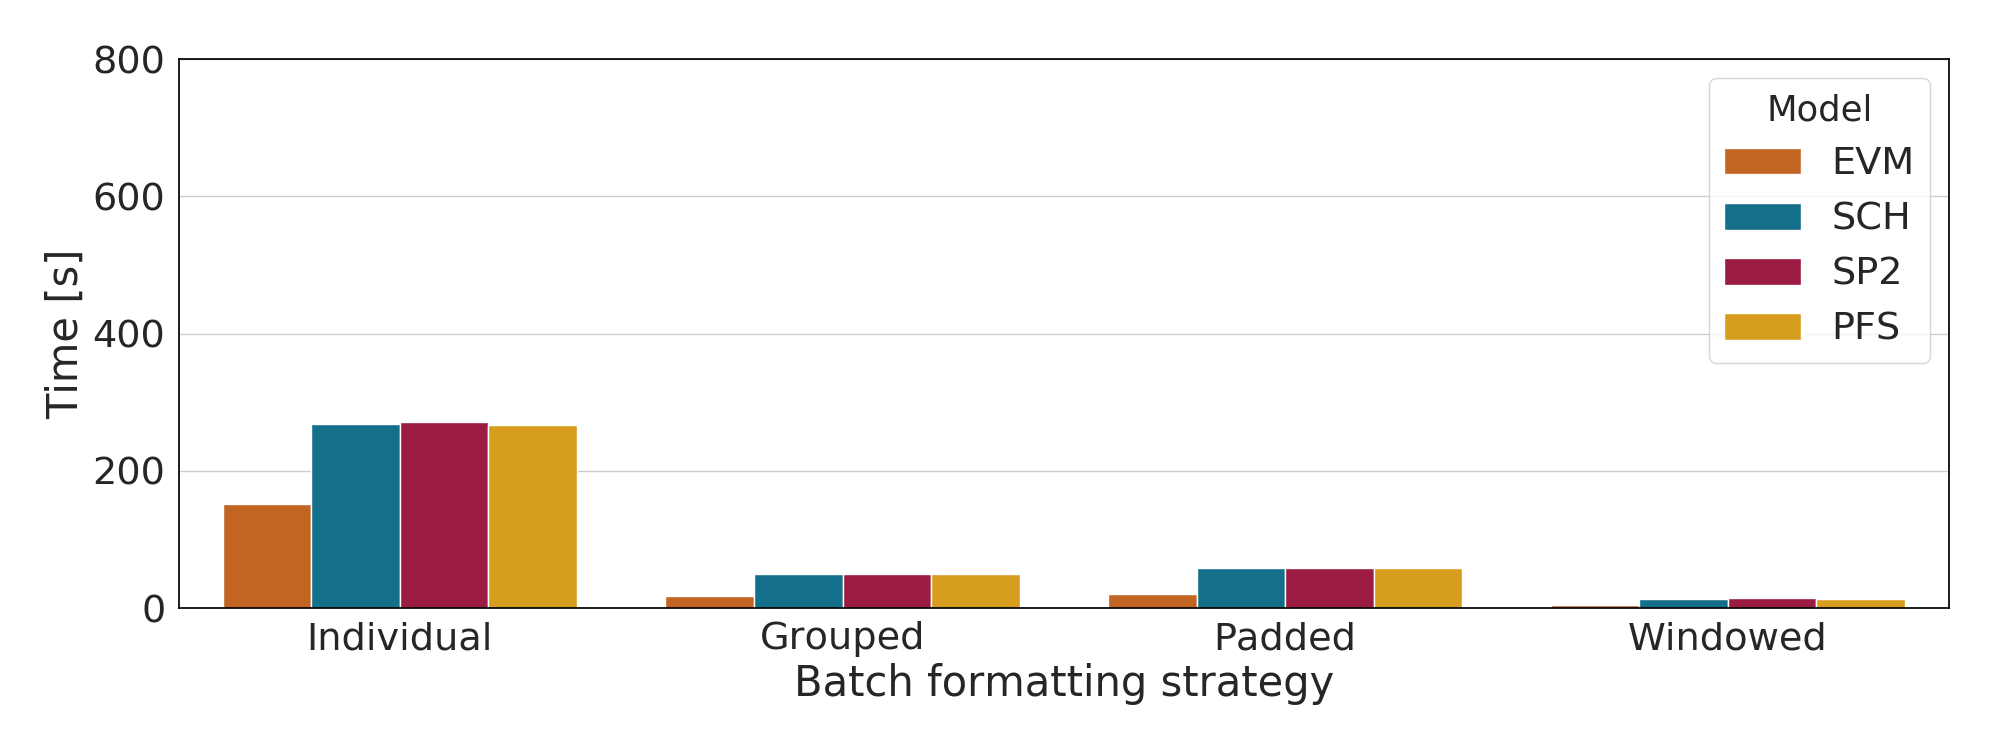
\includegraphics[width=\textwidth]{gfx/bpic2015_1/train_timings.png}
    \caption{Training times measured on BPIC15-1}
    \label{fig:BPIC15-1-training-timings}
\end{figure}
\begin{figure}
    \centering
    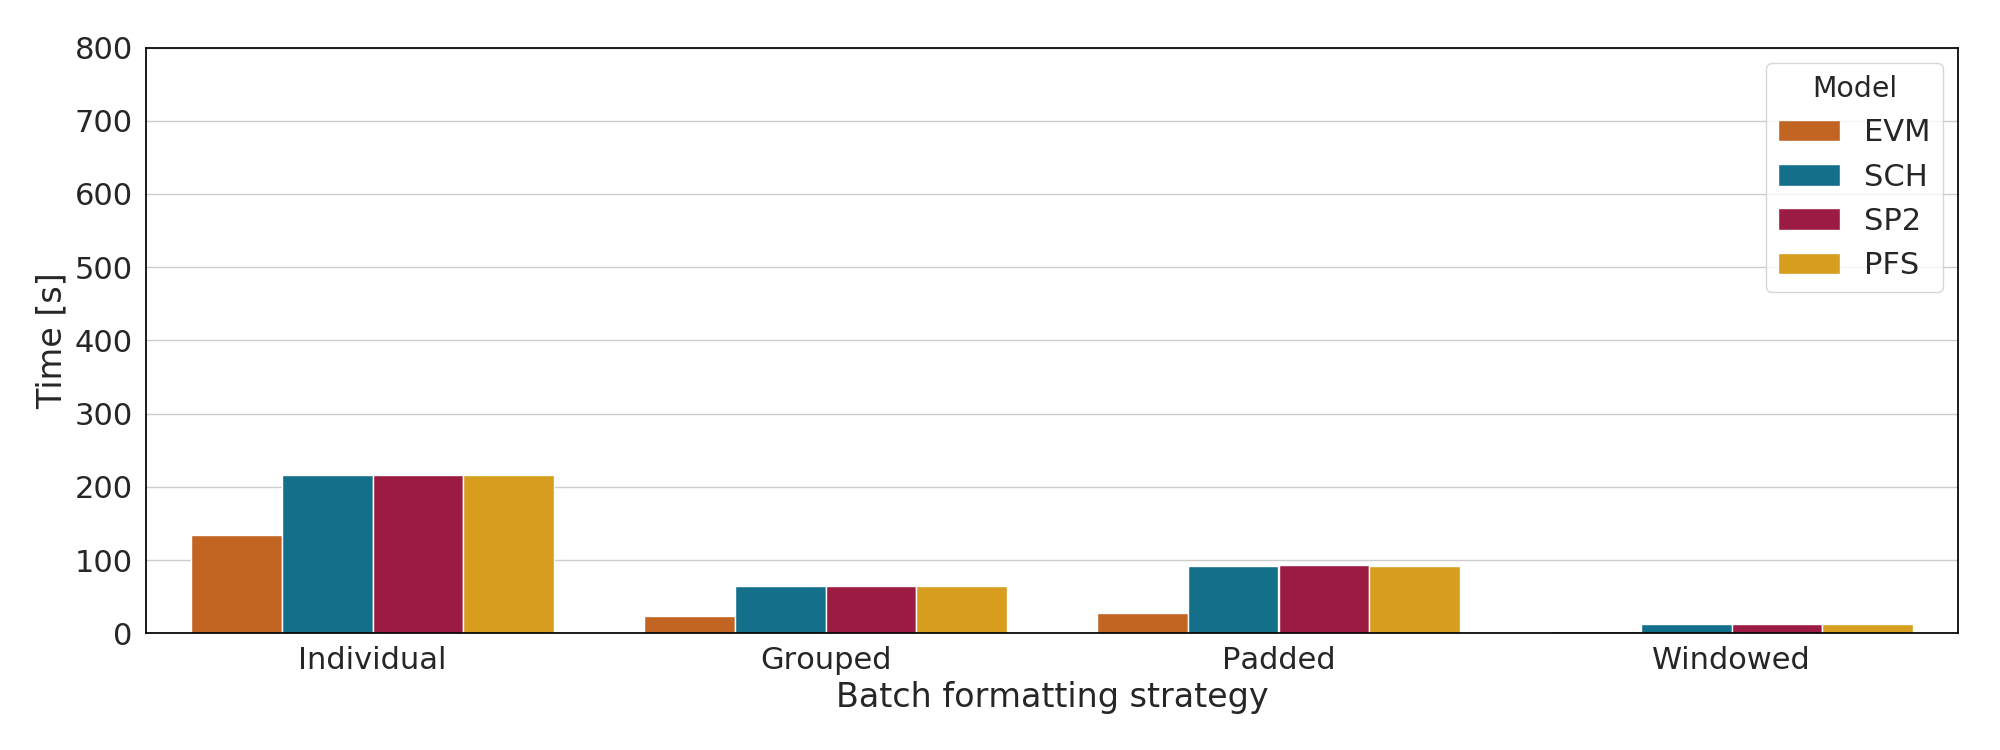
\includegraphics[width=\textwidth]{gfx/bpic2015_2/train_timings.png}
    \caption{Training times measured on BPIC15-2}
    \label{fig:BPIC15-2-training-timings}
\end{figure}
\begin{figure}
    \centering
    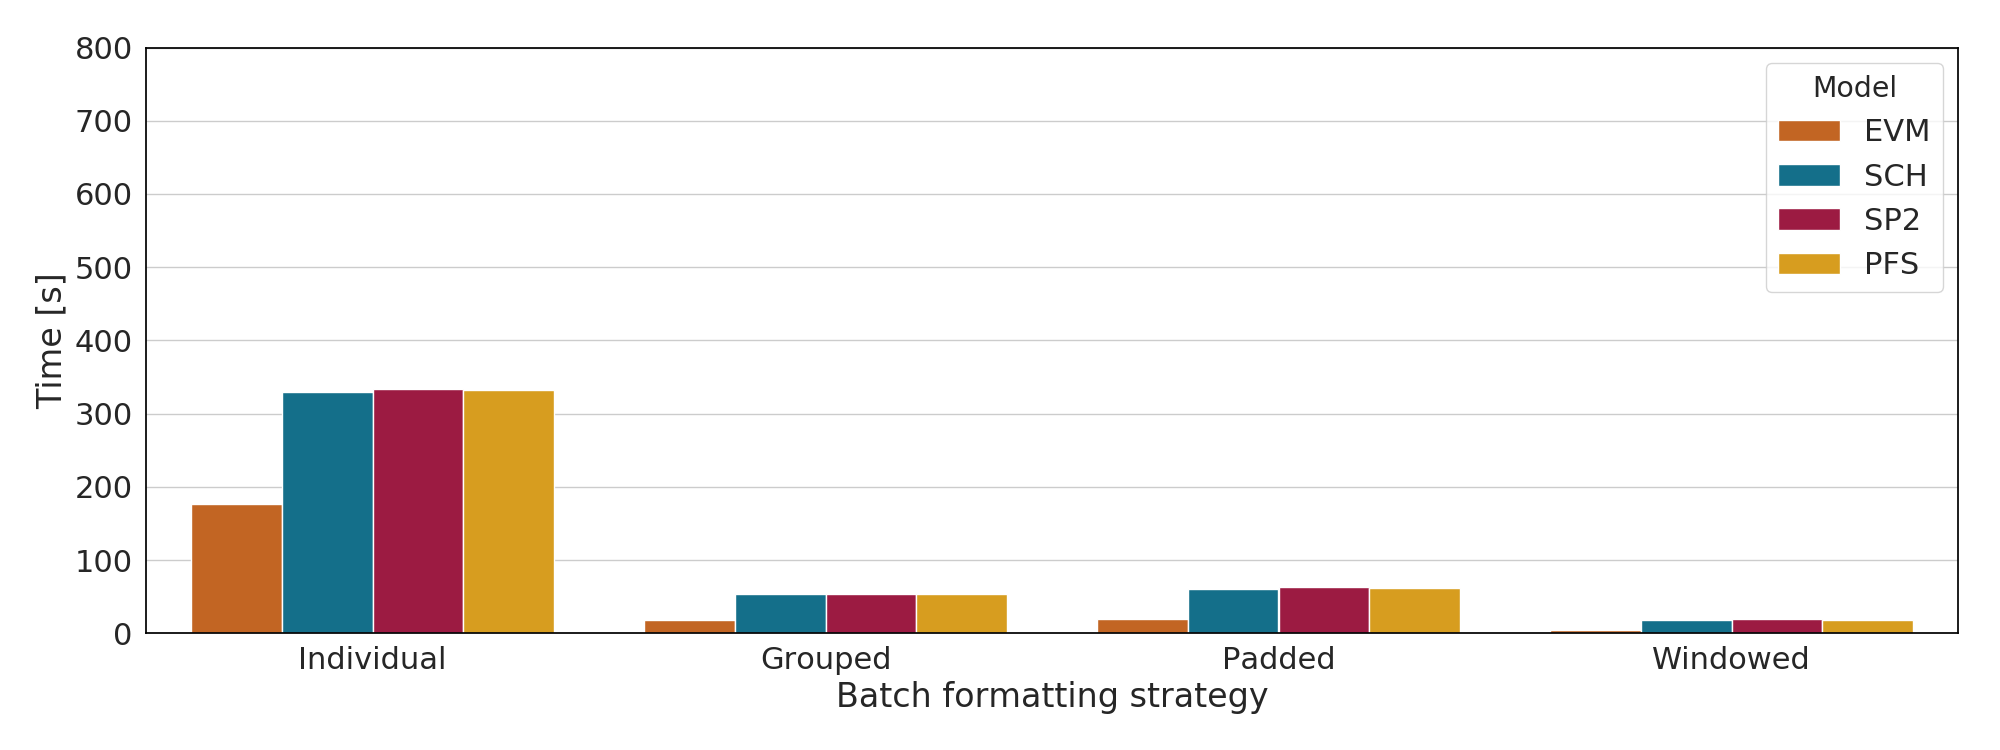
\includegraphics[width=\textwidth]{gfx/bpic2015_3/train_timings.png}
    \caption{Training times measured on BPIC15-3}
    \label{fig:BPIC15-3-training-timings}
\end{figure}
\begin{figure}
    \centering
    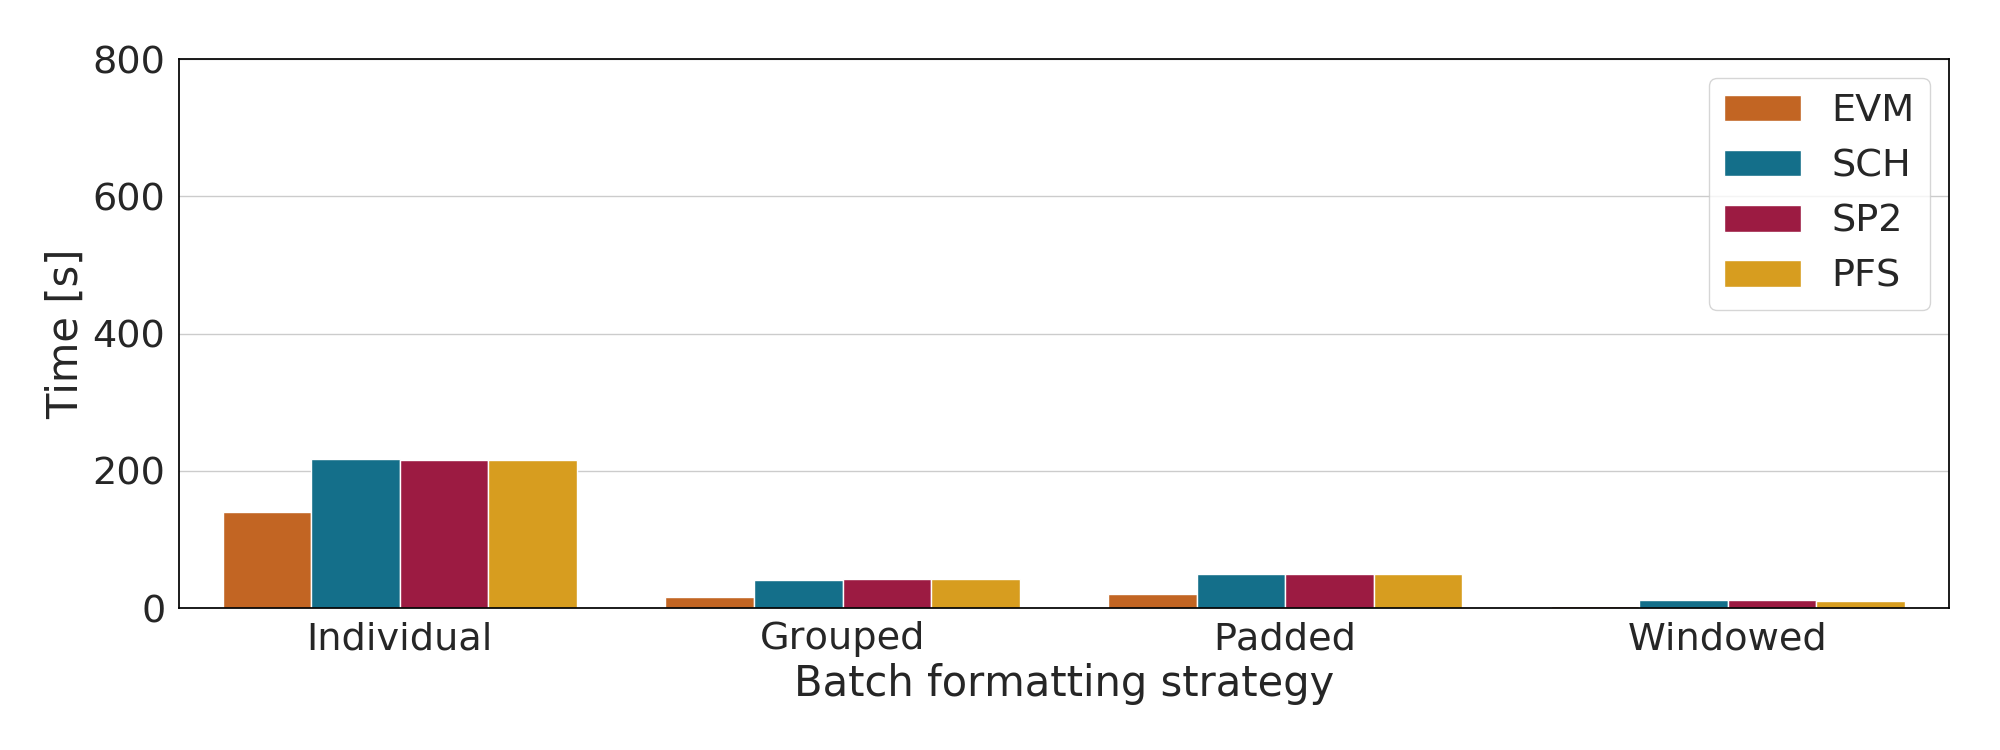
\includegraphics[width=\textwidth]{gfx/bpic2015_4/train_timings.png}
    \caption{Training times measured on BPIC15-4}
    \label{fig:BPIC15-4-training-timings}
\end{figure}
\begin{figure}
    \centering
    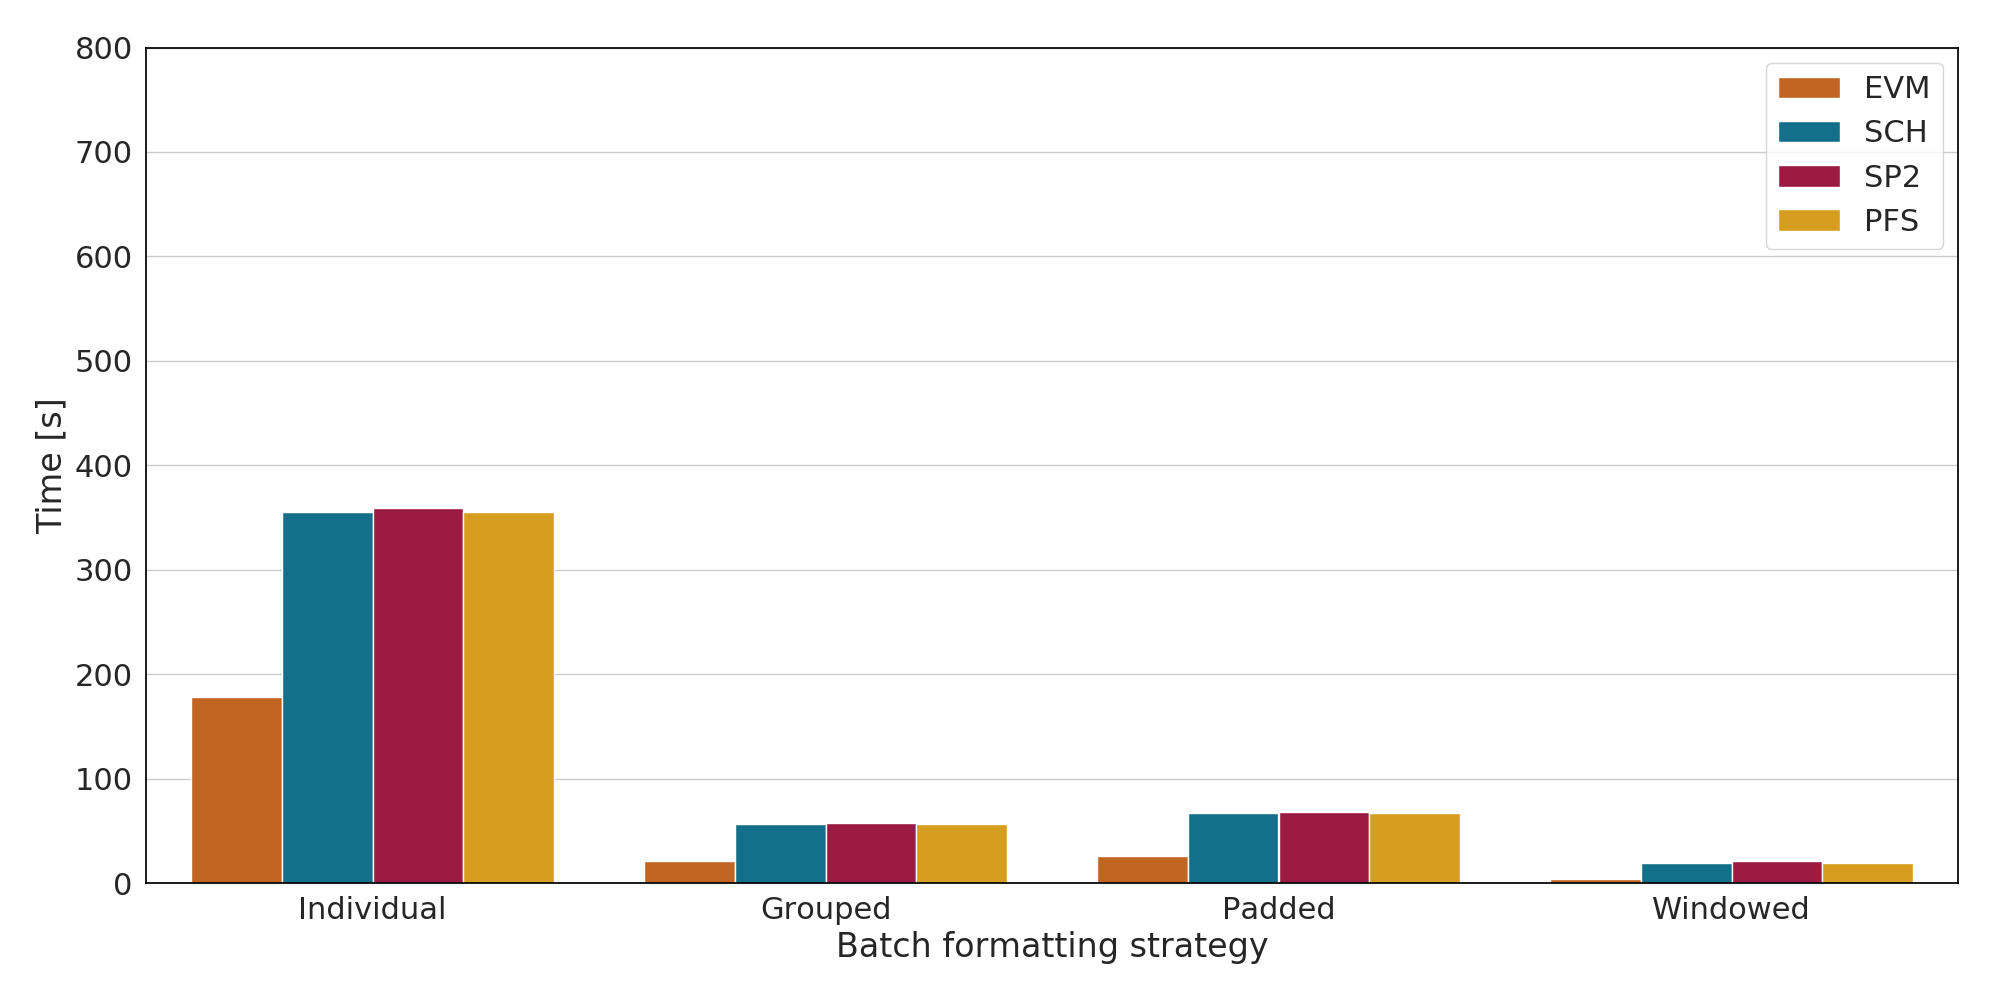
\includegraphics[width=\textwidth]{gfx/bpic2015_5/train_timings.png}
    \caption{Training times measured on BPIC15-5}
    \label{fig:BPIC15-5-training-timings}
\end{figure}

\FloatBarrier
\subsection*{Stability}
As we stressed in the introduction, the stability of a prediction model along the progress of a case greatly impacts the level of trust that users put into the model. \autoref{appendix:evaluation-measurements} contains the figures that illustrate the stability of each model per batching strategy, grouped by dataset. Each figure for a batching strategy and a dataset contains four curves, one for each model. The curves show the model accuracy along the progression of all traces inside the validation set in $5\%$-steps. This subsection explains the results, again per batching strategy.\\

The individual batching strategy not only takes the most time, it also leads to strong differences between the SCH, SP2 and PFS models, even though they are trained on the same data. A good example is the difference between \autoref{fig:bpic15-3-individual-stability} and \autoref{fig:bpic15-3-grouped-stability}. In the latter figure, the curves are a lot closer to each other.

The grouping strategy increases the sample count per batch and this seems to have a harmonizing effect on the results as evidenced by the corresponding figures of all datasets. As noted before, further subdivision of the batches upon exceeding a size threshold could improve accuracy further.

The padded strategy yields results very similar to the grouped strategy, with the exception of BPIC11. In this dataset, the training data had to be trimmed because the padded traces had required too much memory. With the long-tailed distributions in \autoref{appendix:trace-length-distributions} in mind, traces which were longer than $80\%$ of the rest were left out. This reduction of training data most likely causes the reduction in accuracy.

Klinkmüller et al. state that the windowing strategy leads to unstable results~\cite{klinkmuller2018reliablemonitoring}. While this statement seems to be especially true for the longer processes in BPIC11 and BPIC15, the windowing strategy seems to have less of an impact with shorter processes as evidenced with BPIC12. There, all models show a dip towards the end of the trace.\\

Generally, models were expected to become more accurate as the trace neared its end. However this did not prove to be the case. Instead, the accuracy was high when variability in the respective stage of the process was low. For example, processes in BPIC11 always begin similarly, as patients need to be onboarded~\cite{bose2011analysis}. Hence the high accuracies in the beginning. The processes in BPIC12 always end either on an approval or a dismissal of the application, making the model very accurate~\cite{adriansyah2012mining}.

\section{Discussion}
\label{sec:eval:discussion}
After presenting and explaining our findings, we summarize our learnings in this section and compare our findings to the papers mentioned in \autoref{sec:eval:dataset-choice}.\\

First, we were able to confirm Klinkmüller et al.~\cite{klinkmuller2018reliablemonitoring} and their suspicion that windowed batching does not work well for sequence prediction. While it may be a performant strategy to use for time-series prediction, it does not work very well for predicting the future of a single case.

Secondly, we find that the grouping strategy frequently delivers the best results in terms of speed and accuracy. We do realize that it should be iterated upon to include a threshold which limits batches to a maximum size and splits the larger batches accordingly.

Third and lastly, we realize that Embeddings might not be as useful with the currently available datasets as they might simply be too small. The lacking performance of the EVM model and its barely converging loss indicate that this might be the case. All accuracy/loss curves from training are enclosed in \autoref{appendix:loss-curves}, and show that especially for the EVM model, the loss optimization does not work properly.\\

We end the evaluation with a comparison of our best results with the initially mentioned publications based on BPIC12. While Tax et al.~\cite{tax2017} and Evermann et al.~\cite{evermann2016} were able to obtain an accuracy of $0.76$ and $0.768$ respectively, they did not focus on specific cases. Furthermore, Evermann et al. did not use Keras on top of Tensorflow but Tensorflow directly, which enabled him to directly make use of low-level functions. To the best of our knowledge, our implementation sufficiently approximates theirs, but this can be a reason for the bad results. Another very probable reason are the concatenated features used by them~\cite{evermann2016}.

Böhmer et al.~\cite{boehmer2018probability} are able to attain an accuracy of $0.77$. Using the padding strategy, all SCH, SP2 and PFS score above $0.80$, with the SP2 model edging to the best accuracy of $0.82$.
